% FPGA_DAUGHTER_CARD_OPTIONS.tex
% FPGA emulation card for the nanoSoC Ethernet chiplet slot -- revision 2 (K26I slot card).
% Draft for review, 2026-09-30. Build: xelatex FPGA_DAUGHTER_CARD_OPTIONS.tex (twice).
% Self-contained: the figure is inline TikZ. Fonts: Lato and DejaVu Sans Mono if
% installed, else TeX Gyre Heros / Latin Modern Mono.
\documentclass[10pt,a4paper]{article}
\usepackage[a4paper,left=1.8cm,right=1.8cm,top=2.0cm,bottom=2.0cm,headheight=14pt,headsep=0.45cm]{geometry}
\usepackage{fontspec}
\IfFontExistsTF{Lato}{\setmainfont{Lato}[Ligatures=NoCommon]}{\setmainfont{TeX Gyre Heros}}
\IfFontExistsTF{DejaVu Sans Mono}{\setmonofont[Scale=0.82]{DejaVu Sans Mono}}{\setmonofont{Latin Modern Mono}}
\usepackage[table]{xcolor}
\usepackage{booktabs}
\usepackage{array}
\usepackage{tabularx}
\usepackage{enumitem}
\usepackage{titlesec}
\usepackage{fancyhdr}
\usepackage{lastpage}
\usepackage[font=small,labelfont=bf,labelsep=period,skip=4pt]{caption}
\usepackage{float}
\usepackage{needspace}
\usepackage{tikz}
\usetikzlibrary{positioning,arrows.meta,calc,fit,backgrounds}
\usepackage[most]{tcolorbox}
\usepackage{url}
\usepackage[hidelinks]{hyperref}
\def\UrlBreaks{\do\/\do\-\do\.\do\_\do\=\do\?\do\&}
\def\UrlFont{\ttfamily}

\definecolor{accent}{HTML}{1F3A5F}
\definecolor{accent2}{HTML}{2E6DA4}
\definecolor{srcgray}{HTML}{5A6570}
\definecolor{headgray}{HTML}{E3E8EF}
\definecolor{rowgray}{HTML}{F5F7FA}
\definecolor{warn}{HTML}{B03A2E}
\definecolor{ok}{HTML}{2E7D32}
\definecolor{amber}{HTML}{A66300}
\definecolor{gPower}{HTML}{8C8C8C}
\definecolor{gClk}{HTML}{D55E00}
\definecolor{gDbg}{HTML}{0072B2}
\definecolor{gQspi}{HTML}{009E73}
\definecolor{gRmii}{HTML}{E69F00}
\definecolor{gD2d}{HTML}{CC79A7}

% repo citation: \src{path:line}
\DeclareUrlCommand\srcraw{\def\UrlFont{\scriptsize\ttfamily}\def\UrlBreaks{\do\/\do\_\do\-\do\.\do\:\do\,}}
\newcommand\src{\leavevmode\begingroup\color{srcgray}\srcaux}
\newcommand\srcaux[1]{\srcraw{#1}\endgroup}
\DeclareUrlCommand\sig{\def\UrlFont{\ttfamily}\def\UrlBreaks{\do\_\do\/\do\-\do\.\do\,}}
\newcommand\est{\textcolor{amber}{\textsuperscript{est}}}
\newcommand\unc{\textcolor{warn}{\textbf{[unconfirmed]}}}
\newcommand\snip{\textcolor{warn}{[snippet]}}
\newcommand\bdc[1]{\textcolor{warn}{#1}}
\newcommand\okc[1]{\textcolor{ok}{#1}}
\newcommand\amc[1]{\textcolor{amber}{#1}}
\newcommand\R[1]{\textcolor{accent2}{[#1]}}
\newcolumntype{L}{>{\raggedright\arraybackslash}X}
\newcolumntype{P}[1]{>{\raggedright\arraybackslash}p{#1}}
\newcolumntype{C}[1]{>{\centering\arraybackslash}p{#1}}

\titleformat{\section}{\large\bfseries\color{accent}}{\thesection}{0.6em}{}
\titlespacing*{\section}{0pt}{9pt}{3pt}
\titleformat{\subsection}{\normalsize\bfseries\color{accent}}{\thesubsection}{0.5em}{}
\titlespacing*{\subsection}{0pt}{6pt}{2pt}
\setlength{\parindent}{0pt}
\setlength{\parskip}{3pt}
\setlist{nosep,leftmargin=1.2em,topsep=1pt}
\renewcommand{\arraystretch}{1.12}

\pagestyle{fancy}
\fancyhf{}
\fancyhead[L]{\small\color{srcgray}FPGA emulation card for the nanoSoC Ethernet chiplet slot}
\fancyhead[R]{\small\color{srcgray}Draft for review, 2026-09-30}
\fancyfoot[C]{\small\color{srcgray}\thepage\ of \pageref{LastPage}}
\renewcommand{\headrulewidth}{0.3pt}

\newtcolorbox{verdict}{colback=accent2!6,colframe=accent,boxrule=0.6pt,arc=2pt,left=5pt,right=5pt,top=3pt,bottom=3pt}
\newtcolorbox{caveat}{colback=warn!4,colframe=warn!70,boxrule=0.5pt,arc=2pt,left=5pt,right=5pt,top=2pt,bottom=2pt}

\begin{document}

\begin{center}
{\LARGE\bfseries\color{accent} FPGA emulation card for the nanoSoC Ethernet chiplet slot}\\[3pt]
{\large Draft for review \quad\textbar\quad 2026-09-30 \quad\textbar\quad revision 2: K26I slot card}\\[2pt]
{\small\color{srcgray} For the bring-up and PCB engineers. Device: nanoSoC Ethernet chiplet rc4-20260829 (TSMC 65\,nm). Interface: slot contract v1, 120-position HSEC8.}
\end{center}
\vspace{-2pt}

\begin{verdict}
\textbf{Verdict: build a Kria K26I slot card (CARD\_ID 001).} It plugs into the same slot as the bonded-die card, so the two are interchangeable, as the user requires.
\begin{itemize}
\item \textbf{Why the K26I:}
  \begin{itemize}
  \item It is the same XCK26 device as the proven KR260 build. The whole chiplet (58k LUTs, including TideLink) uses 51\,\%.
  \item Its 69 HDIO at 3.3\,V carry all 48 slot signals. Banks 43 + 44 hold exactly 48.
  \item The nanoSoC FPGA Toolkit already supports \texttt{zynqmp}.
  \item It is in stock: 112 at Mouser UK, \pounds439.21, on 2026-09-30. The K26C had 0.
  \end{itemize}
  The K26I differs from the K26C only in temperature grade and shock/vibration qualification (DS987 v1.2 tables 1, 22, 25). Build for \texttt{xck26-sfvc784-2LV-i}.
\item \textbf{Now:} develop the emulator bitstream on the lab's KR260s, which use the same device.
  \begin{itemize}
  \item Undo the QSPI/HOSTIO4 tie-offs.
  \item Take CLK from a pin.
  \item Use the silicon boot ROMs.
  \item Start from the HAPS-SX board top.
  \end{itemize}
\item \textbf{Optional:} a KR260 + paddle adapter (36 IO; no TideLink). Build it only if the motherboard is ready well before the K26 card.
\item \textbf{Effort}\est:
  \begin{itemize}
  \item card: 20--26 engineer-days plus 3--4 weeks of fabrication and assembly;
  \item bitstream: 16--22 engineer-days, in parallel on a KR260;
  \item \textbf{total: about 36--48 engineer-days, 2--3 months elapsed.}
  \end{itemize}
\end{itemize}
\end{verdict}

\begin{table}[H]\centering\footnotesize
\caption{Options. ``Fits'' = post-route LUT use of 75\,\% or less for the whole chiplet (58k LUTs). \est{} marks my estimates.}
\begin{tabularx}{\textwidth}{@{}P{3.3cm}P{1.7cm}P{1.9cm}P{1.5cm}P{2.3cm}L@{}}
\toprule
\rowcolor{headgray}Option & Fits? & 3.3\,V IO & Same slot as die card? & Stock, price (2026-09-30) & Decision\\
\midrule
\rowcolor{ok!10}\textbf{K26I SOM on slot carrier} & \okc{51\,\%} & 69 HDIO & \okc{yes} & 112 at Mouser UK, \pounds439 & \okc{\textbf{Chosen.}} Proven device; all 48 signals; toolkit supports it.\\
K26C SOM on slot carrier & \okc{51\,\%} & 69 HDIO & \okc{yes} & 0 in stock, \pounds353 & \amc{Same card.} Use it if stock returns; 0--85\,$^\circ$C only.\\
Trenz TE0712 A7-200T on carrier & \okc{43\,\%} & 158 HR & \okc{yes} & 0 in stock, \texteuro289 net & \amc{Fallback.} Lower power. The toolkit's \texttt{bin\_style} is \{zynq7, zynqmp, none\} (\src{fpga/fpga-toolkit/part/pack_schema.tcl:494}), so booting an Artix-7 from SPI flash needs an extension.\\
K24 SOM on carrier & \bdc{82\,\%} of 70.6k & 23 HDIO & yes & --- & \bdc{Rejected.} Too few 3.3\,V IO; the 1.8\,V HPIO would need level shifters (DS985).\\
Kria on the motherboard & \okc{51\,\%} & 69 & \bdc{no} & --- & \bdc{Rejected.} Breaks interchangeability.\\
KR260 + paddle adapter & \okc{51\,\%} & 36 used & yes (cabled) & owned & \amc{Optional.} Only if the motherboard is ready well before the card. No TideLink or I2C.\\
Nexys Video + FMC cable & \okc{43\,\%} & 68 LA & cabled & \$711 & \bdc{Not pursued.} A bench cable, not a slot card.\\
\bottomrule
\end{tabularx}
\end{table}

\section{Design size and the existing FPGA builds}

\begin{table}[H]\centering\footnotesize
\caption{Measured FPGA resource use (BRAM in 36\,Kb tiles). Sources are under the table.}
\begin{tabular}{@{}p{5.6cm}p{1.9cm}rrrrp{2.6cm}@{}}
\toprule
\rowcolor{headgray}Build & Device & LUT & FF & BRAM & DSP & SoC clock, slack\\
\midrule
\textbf{[1]} KR260 ``landed'', whole design & xck26-2LV & 59,851 & 54,337 & 32.5 & 7 & 25.0\,MHz, +12.37\,ns\\
\quad of which \sig{nanosoc_eth_chiplet} & & 58,031 & 52,414 & 32.5 & 7 & \\
\quad\quad SoC (\sig{u_soc}) & & 28,212 & 19,342 & 28.5 & 6 & \\
\quad\quad TideLink & & 23,672 & 27,673 & 4 & 1 & \\
\quad\quad TideChart + APB bridges + D2D decode & & 6,170 & 5,364 & 0 & 0 & \\
\textbf{[2]} HAPS-SX, \texttt{PHY=rmii} & xcvu19p-2 & 57,617 & 51,503 & 41 & 7 & 25\,MHz; hold fails\\
\textbf{[3]} PYNQ-Z2 multicore SoC, \textbf{no TideLink} & xc7z020-1 & 27,958 & 19,827 & 31.5 & 6 & 25\,MHz, +0.58\,ns\\
\bottomrule
\end{tabular}\\[2pt]
\begin{minipage}{\textwidth}\scriptsize\color{srcgray}\raggedright
\textbf{[1]} \src{fpga/build/landed/reports/utilization_impl.rpt:36,41,109,125}; \src{utilization_hier_impl.rpt:351,357,1041,1033,1032,1509,356}; \src{timing_summary.rpt:197,215}.
\textbf{[2]} \src{~/SoCLabs/HAPS-work/fpga/haps-sx/build/vivado_out/post_route_util.rpt:40,113}; \src{README.md:19-27}.
\textbf{[3]} \src{nanosoc-multicore-system/imp/fpga/project/pynq-z2/nanosoc_multicore_project.runs/impl_1/nanosoc_multicore_design_wrapper_utilization_placed.rpt:35,40,106}; \src{..._timing_summary_routed.rpt:154,169}.
\end{minipage}
\end{table}

\begin{itemize}
\item \textbf{Size.} The whole chiplet is about 58k LUTs, and TideLink + TideChart are about 30k of that. The ``131k'' figure for the KR260 is its primitive-cell count. On the K26 (117,120 LUTs) it is 51\,\% full; on the K24 (70,560 LUTs, DS985) it would be 82\,\%. Memory is small: 32.5 of 144 BRAM tiles.
\item \textbf{Clock.} Every FPGA build runs the SoC at 25\,MHz. On the K26 there is +12.4\,ns of slack at 25\,MHz, so about 35\,MHz may be possible\est. The RMII domain runs directly from the 50\,MHz REF\_CLK with 18.5\,ns of slack (\src{timing_summary.rpt:211}).
\item \textbf{The KR260 build cannot go into the slot as it is.}
  \begin{itemize}
  \item The SoC clock and reset come from the PS: PL0 100\,MHz through a clk\_wiz to 25\,MHz (\src{tidelink/fpga/targets/kr260-eth-chiplet/tidelink_design.tcl:95,108,166}).
  \item QSPI, SPI and HOSTIO4 are tied off in the packaged IP wrapper (\src{tidelink/fpga/vivado_ip/nanosoc_eth_chiplet_vivado_wrapper.v:257-269}).
  \item The eth ROM is \texttt{smoke\_remap}, not silicon's \texttt{stage0}. 172 of 320 words differ, and \texttt{stage0} copies from QSPI flash and halts without it (\src{docs/bringup/ASIC_FIRST_SILICON_HOSTIO_PROCEDURE.md:123}).
  \item IMEM is preloaded with \sig{RAM_PRELOAD} (\src{tidelink/fpga/vivado_ip/nanosoc_eth_chiplet_filelist.tcl:171-225}).
  \end{itemize}
\item \textbf{The HAPS-SX board top already has what the slot needs.}
  \begin{itemize}
  \item It wires QSPI, HOSTIO4, SWD and RMII (\src{HAPS-work/fpga/haps-sx/vsrc/nanosoc_eth_chiplet_haps_sx.sv:95-156}).
  \item It loads the rc4 silicon eth ROM; CPU1's ROM already matches silicon (\src{HAPS-work/fpga/haps-sx/Makefile:206-215}).
  \item It times QSPI SCK as HCLK/2, like silicon at boot (\src{README.md:305-310}).
  \end{itemize}
  Its hold failures (\src{README.md:19-27}) must be re-checked on the K26.
\end{itemize}

\section{K26I slot card: what to build}

\begin{figure}[H]\centering
\resizebox{\textwidth}{!}{%
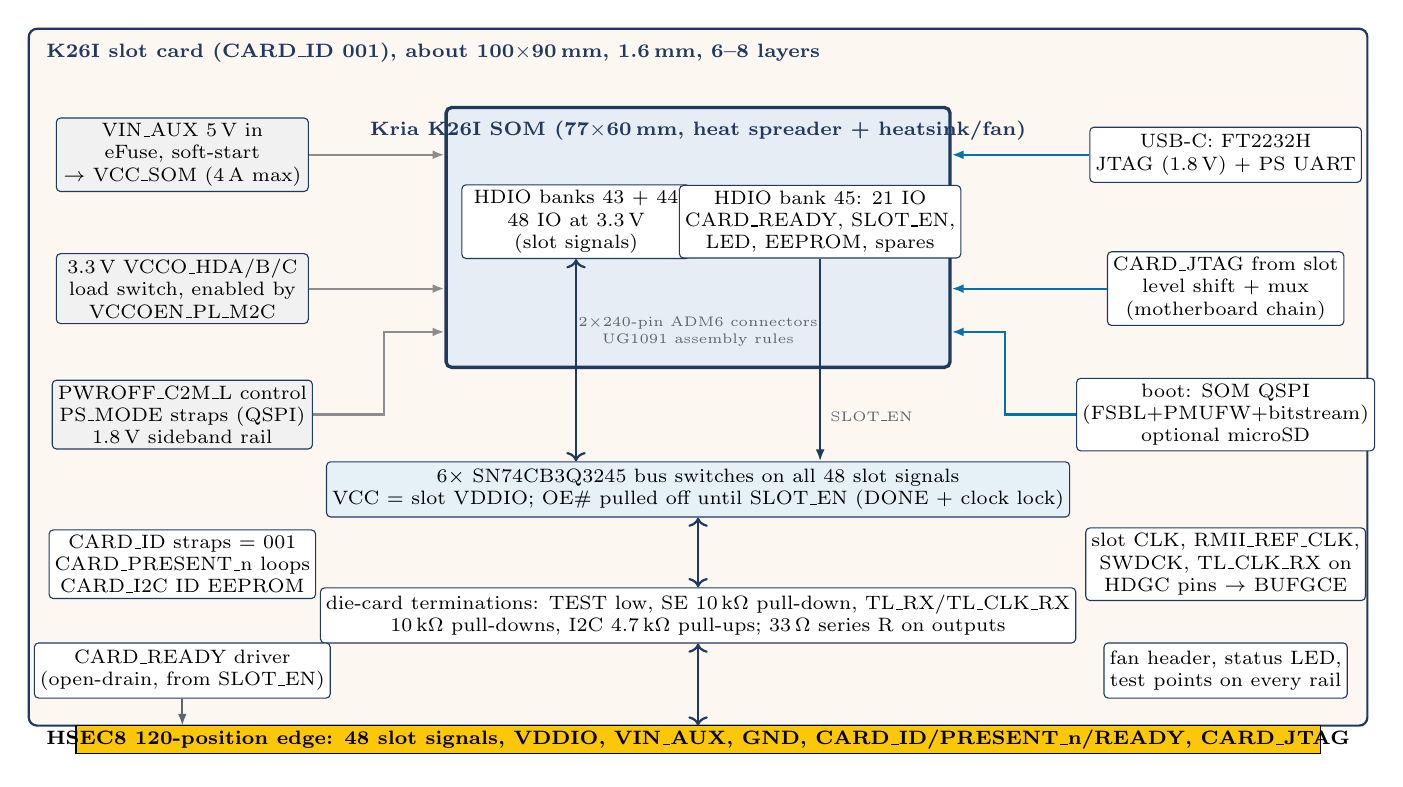
\begin{tikzpicture}[font=\scriptsize,
  blk/.style={draw=accent,rounded corners=1.5pt,fill=white,align=center,inner sep=2pt,minimum height=7mm},
  pw/.style={blk,fill=gPower!12},
  sw/.style={blk,fill=gDbg!10},
  som/.style={draw=accent,very thick,rounded corners=2pt,fill=accent2!12,align=center},
  note/.style={font=\tiny,text=srcgray,align=center},
  lab/.style={font=\scriptsize\bfseries,text=accent},
  wire/.style={-{Latex[length=1.5mm]},thick}]
% card outline (paddle card, HSEC8 fingers at the bottom)
\draw[draw=accent,thick,fill=gClk!5,rounded corners=3pt] (0,0.35) rectangle (17,9.2);
\node[lab,anchor=north west] at (0.1,9.15) {K26I slot card (CARD\_ID 001), about 100$\times$90\,mm, 1.6\,mm, 6--8 layers};
\draw[fill=yellow!60!orange] (0.6,0.0) rectangle (16.4,0.35);
\node[font=\scriptsize\bfseries] at (8.5,0.17) {HSEC8 120-position edge: 48 slot signals, VDDIO, VIN\_AUX, GND, CARD\_ID/PRESENT\_n/READY, CARD\_JTAG};
% SOM
\node[som,minimum width=6.4cm,minimum height=3.3cm] (som) at (8.5,6.55) {};
\node[lab,anchor=north] at (8.5,8.15) {Kria K26I SOM (77$\times$60\,mm, heat spreader + heatsink/fan)};
\node[blk,minimum width=2.9cm] (hd) at (6.95,6.75) {HDIO banks 43 + 44\\48 IO at 3.3\,V\\(slot signals)};
\node[blk,minimum width=2.9cm] (hd45) at (10.05,6.75) {HDIO bank 45: 21 IO\\CARD\_READY, SLOT\_EN,\\LED, EEPROM, spares};
\node[note] at (8.5,5.35) {2$\times$240-pin ADM6 connectors\\UG1091 assembly rules};
% power column (left)
\node[pw,minimum width=3.2cm] (efuse) at (1.95,7.6) {VIN\_AUX 5\,V in\\eFuse, soft-start\\$\rightarrow$ VCC\_SOM (4\,A max)};
\node[pw,minimum width=3.2cm] (vcco) at (1.95,5.9) {3.3\,V VCCO\_HDA/B/C\\load switch, enabled by\\VCCOEN\_PL\_M2C};
\node[pw,minimum width=3.2cm] (pwroff) at (1.95,4.3) {PWROFF\_C2M\_L control\\PS\_MODE straps (QSPI)\\1.8\,V sideband rail};
\draw[wire,gPower] (efuse.east) -- (som.west |- efuse.east);
\draw[wire,gPower] (vcco.east) -- (som.west |- vcco.east);
\draw[wire,gPower] (pwroff.east) -- ++(0.9,0) |- (som.west |- 5.35,5.35);
% debug/boot column (right)
\node[blk,minimum width=3.0cm] (usb) at (15.2,7.6) {USB-C: FT2232H\\JTAG (1.8\,V) + PS UART};
\node[blk,minimum width=3.0cm] (cj) at (15.2,5.9) {CARD\_JTAG from slot\\level shift + mux\\(motherboard chain)};
\node[blk,minimum width=3.0cm] (sd) at (15.2,4.3) {boot: SOM QSPI\\(FSBL+PMUFW+bitstream)\\optional microSD};
\draw[wire,gDbg] (usb.west) -- (som.east |- usb.west);
\draw[wire,gDbg] (cj.west) -- (som.east |- cj.west);
\draw[wire,gDbg] (sd.west) -- ++(-0.9,0) |- (som.east |- 5.35,5.35);
% bus switches and terminations
\node[sw,minimum width=6.4cm] (bsw) at (8.5,3.35) {6$\times$ SN74CB3Q3245 bus switches on all 48 slot signals\\VCC = slot VDDIO; OE\# pulled off until SLOT\_EN (DONE + clock lock)};
\draw[wire,accent,<->] (hd.south) -- (hd.south |- bsw.north);
\draw[wire,accent] (hd45.south) -- node[pos=0.78,right,note,align=left]{SLOT\_EN} (hd45.south |- bsw.north);
\node[blk,minimum width=6.4cm] (term) at (8.5,1.75) {die-card terminations: TEST low, SE 10\,k$\Omega$ pull-down, TL\_RX/TL\_CLK\_RX\\10\,k$\Omega$ pull-downs, I2C 4.7\,k$\Omega$ pull-ups; 33\,$\Omega$ series R on outputs};
\draw[wire,accent,<->] (bsw.south) -- (term.north);
\draw[wire,accent,<->] (term.south) -- (8.5,0.35);
\node[blk,minimum width=3.2cm] (id) at (1.95,2.4) {CARD\_ID straps = 001\\CARD\_PRESENT\_n loops\\CARD\_I2C ID EEPROM};
\node[blk,minimum width=3.2cm] (rdy) at (1.95,1.05) {CARD\_READY driver\\(open-drain, from SLOT\_EN)};
\draw[wire,srcgray] (rdy.south) -- (rdy.south |- 0.35,0.35);
\node[blk,minimum width=3.0cm] (clk) at (15.2,2.4) {slot CLK, RMII\_REF\_CLK,\\SWDCK, TL\_CLK\_RX on\\HDGC pins $\rightarrow$ BUFGCE};
\node[blk,minimum width=3.0cm] (fan) at (15.2,1.05) {fan header, status LED,\\test points on every rail};
\end{tikzpicture}
}
\caption{Block diagram of the K26I slot card. Slot signals run from HDIO banks 43 and 44, through Ioff-rated bus switches powered from slot VDDIO, to the edge fingers. The die-card terminations sit on the slot side of the switches, so the slot nets look the same whichever card is fitted.}
\end{figure}

\begin{table}[H]\centering\footnotesize
\caption{Carrier requirements. ``DS987'' and ``UG1091'' items were read from AMD documents; the rest are design choices for this card.}
\begin{tabularx}{\textwidth}{@{}P{2.8cm}LP{2.2cm}@{}}
\toprule
\rowcolor{headgray}Area & Requirement & Source\\
\midrule
SOM power & VCC\_SOM is 5\,V (4.75--5.25\,V, 50\,mV p-p max noise), 4\,A max. Fed from slot VIN\_AUX through an eFuse with soft-start. PWROFF\_C2M\_L (active low, pulled up to 5\,V on the SOM) powers the SOM down and, when released, starts its power-on sequence; the carrier drives it from a power-on-reset / host-controlled signal. & DS987 table 17 and ``Power Management Signals''; UG1091 ``Power Sequencing''\\
HDIO bank power & The carrier supplies VCCO\_HDA/HDB/HDC (1.2--3.3\,V, 1\,A each) and must enable them only after the SOM asserts VCCOEN\_PL\_M2C. Here: a 3.3\,V rail from VIN\_AUX through a load switch driven by VCCOEN\_PL\_M2C. The VCCO tolerance at the connector is +3\,\%/--2\,\%. VCCOEN\_PS\_M2C gates the PS-peripheral rails (UART, microSD) the same way. & DS987 table 17; UG1091 ``PL Power Up Behavior''\\
Connectors & 2$\times$ Samtec ADM6-60-01.5-L-4-2-A (carrier side; 0.635\,mm, 4-row, 240 positions each). UG1091 gives placement, distance-tolerance, stencil and reflow rules: use an assembler who has built Kria carriers. & UG1091 ``SOM Connector Overview''\\
Boot & The SOM holds 512\,Mb QSPI and 16\,GB eMMC. PS\_MODE[3:0] are pulled up on the SOM; strap 0010 (QSPI) with 0\,$\Omega$ to GND. Own BOOT.BIN (FSBL + PMUFW + bitstream) in QSPI, so no Linux is needed. Optional microSD on MIO. & DS987 table 6, ``Sideband Signals''\\
Debug & SOM JTAG pins are 1.8\,V sideband. FT2232H USB (JTAG + PS UART) on a USB-C port, level-shifted. The slot CARD\_JTAG (VREF = VDDIO) is buffered and muxed into the same chain. & DS987 ``Sideband Signals''; contract v1\\
Slot IO isolation & 6$\times$ SN74CB3Q3245 (8-bit, 4\,$\Omega$, 500\,MHz, Ioff) on all 48 signals. VCC comes from slot VDDIO. OE\# is pulled to ``off'' until the bitstream drives SLOT\_EN (DONE + clock lock), which also releases CARD\_READY. Nothing reaches the slot during configuration or while VDDIO is off. & TI product page; contract v1\\
Terminations & The die-card set on the slot side: TEST low, SE 10\,k$\Omega$ pull-down, TL\_RX[7:0]/TL\_CLK\_RX 10\,k$\Omega$ pull-downs, I2C 4.7\,k$\Omega$ pull-ups, 33\,$\Omega$ series R on outputs. & contract v1\\
Identity & CARD\_ID straps 001, both CARD\_PRESENT\_n loops, CARD\_READY open-drain, CARD\_I2C ID EEPROM, status LED. & contract v1\\
Pins and clocks & 48 slot signals on HDIO banks 43 + 44 (24 + 24). Card control on bank 45 (21 IO). CLK, RMII\_REF\_CLK, SWDCK and TL\_CLK\_RX on HDGC pins. & DS987 pin table\\
Thermal, mechanics & The SOM (77$\times$60$\times$10.9\,mm, 58\,g) has a heat spreader, and the cooling solution attaches to it. Fit a heatsink + fan (fan header). Card up to about 100$\times$90\,mm; the motherboard provides a keep-out volume and a card guide or bracket; same keying as the die card; no hot-plug. & DS987 tables 22--23; contract v1\\
\bottomrule
\end{tabularx}
\end{table}

\begin{table}[H]\centering\footnotesize
\caption{Card effort (my estimates, one experienced PCB engineer).}
\begin{tabularx}{\textwidth}{@{}LP{3.2cm}@{}}
\toprule
\rowcolor{headgray}Item & Effort\est\\
\midrule
Schematic: power and sequencing, SOM connectors, bus switches, JTAG/UART, boot straps, terminations, ID & 6--8\,d\\
Layout: 6--8 layers, ADM6 fan-out, 1.6\,mm paddle with hard-gold HSEC8 fingers, heatsink keep-outs & 8--10\,d\\
Fabrication and assembly (fine-pitch connectors, gold fingers) & 3--4 weeks elapsed\\
Carrier bring-up: rails, PWROFF / VCCOEN sequence, JTAG, QSPI boot, CARD\_READY & 4--6\,d\\
Mechanical: heatsink/fan choice, card guide agreed with the motherboard & 2\,d\\
\textbf{Card total} & \textbf{20--26\,d + 3--4\,wk}\\
\bottomrule
\end{tabularx}
\end{table}

\section{RTL and bitstream work (start now on a KR260)}

\begin{table}[H]\centering\footnotesize
\begin{tabularx}{\textwidth}{@{}P{3.3cm}LP{1.4cm}@{}}
\toprule
\rowcolor{headgray}Item & Content & Effort\est\\
\midrule
Board top & Fork the HAPS-SX top for the XCK26. Keep the PS only for configuration and debug. Remove the PS AXI-to-AHB backdoor, which is tied idle on silicon, and the tie-offs in \src{nanosoc_eth_chiplet_vivado_wrapper.v:257-269}. & 3--4\,d\\
Clocking & Slot CLK on an HDGC pin. At 25\,MHz (contract v1 option) drive a BUFGCE directly with no MMCM, so CLK gating and NRST release match silicon. At 50/100\,MHz use an MMCM $\div$2/$\div$4 and hold reset until lock. The HDGC$\rightarrow$MMCM route must be checked in Vivado, because the MMCMs sit in the HP columns (\unc). RMII\_REF\_CLK drives the MAC domain directly. & 2--3\,d\\
Silicon ROMs & eth ROM = \texttt{eth\_ss\_bootrom.rc4.bintxt} (as \src{HAPS-work/fpga/haps-sx/Makefile:206-215}); CPU1 ROM already matches silicon. Drop \sig{RAM_PRELOAD}. Firmware built for 25\,MHz (\sig{NS_INCR} = 40, \sig{NANOSOC_SYS_CLK_FREQ_HZ}). & 1--2\,d\\
Pad wrapper & \texttt{nanosoc\_eth\_chiplet\_pads\_fpga.v}: mirror \src{ASIC/tech_wrappers/tsmc65/nanosoc_eth_chiplet_pads.v} with IOBUF and PULLUP/PULLDOWN matching rc4's pull states. Keep \sig{nanosoc_eth_chiplet_bscan} (\src{:372-384}) so IDCODE, BYPASS and EXTEST work from the motherboard JTAG header. & 3--5\,d\\
Board packs & \texttt{fpga/board/kr260-slotdev/board.tcl} (KR260 pins, for development now) and \texttt{fpga/board/k26i-slot/board.tcl}: \texttt{part xck26-sfvc784-2LV-i}, \texttt{bin\_style zynqmp}, \texttt{deploy\_style jtag}, SOM-only \texttt{board\_part} (the K26I board-file name is \unc). Pin XDC for 48 + control signals. & 2--3\,d\\
Bring-up against the motherboard & Flash-boot from the motherboard QSPI with a \texttt{mkflash.sh} image; HOSTIO4 suite; RMII ping; TideLink register reads with the link down; CARD\_READY / NRST sequencing. & 5\,d\\
\bottomrule
\end{tabularx}
\end{table}

\section{Slot contract v1: changes adopted}
These supersede v0. All are now part of the contract, not proposals.
\begin{enumerate}[leftmargin=1.5em]
\item \textbf{Card types:} 000 die card, \textbf{001 K26I FPGA card}, 010 packaged die, 111 empty. Every card uses the same 120-position HSEC8 and the same keying. No hot-plug: all rails off before inserting or removing a card.
\item \textbf{VIN\_AUX:} 5\,V at 4\,A or more continuous, on at least 6 contacts (HSEC8 is about 2.8\,A per pin \snip, derated). Supplied through an eFuse with an INA228. The die card leaves it unconnected.
\item \textbf{VDDIO} is on for every card type. The FPGA card uses it to power its slot-side bus switches.
\item \textbf{CARD\_READY:} open-drain, card to motherboard, pulled up on the motherboard. The FPGA card releases it after configuration and slot-IO enable; the die card straps it ready. The host MCU waits for it before releasing NRST.
\item \textbf{Card JTAG on spare pins:} TCK, TMS, TDI, TDO and VREF. The FPGA card also keeps its own USB-JTAG/UART.
\item \textbf{25\,MHz CLK option} on the motherboard oscillator, alongside 50/100\,MHz with OE.
\item \textbf{VDD\_CORE dummy load} (DNP) on the \emph{motherboard}, so the core supply can be tested with the FPGA card fitted.
\item \textbf{Rules for every card:} die-card terminations and series resistors; the FPGA card isolates its slot IO with bus switches until configured.
\item \textbf{Mechanics:} FPGA card up to about 100$\times$90\,mm; a keep-out volume and card support on the motherboard.
\end{enumerate}

\section{Open questions}
\begin{enumerate}[leftmargin=1.5em]
\item The HDGC$\rightarrow$MMCM route on the K26 at 50/100\,MHz. If it fails, run the FPGA card only with the 25\,MHz CLK.
\item K26 power draw with this design. No \texttt{report\_power} exists; DS987 gives only the 4\,A maximum. Measure it on a KR260 to size the heatsink and confirm the VIN\_AUX margin.
\item Board files for a custom K26I carrier: the SOM-only \texttt{board\_part} name, and whether the factory QSPI boot firmware expects a carrier ID EEPROM. The plan is to write our own BOOT.BIN.
\item The KR260 bank 45 (PMOD1/2) fault (\src{ASIC_FIRST_SILICON_HOSTIO_PROCEDURE.md:165}): is it on the SOM or on the carrier? The card puts only control signals on bank 45.
\item The HSEC8 per-pin current rating (\snip) and the Mouser K26I stock figure (from contract v1) should be re-read from the datasheet and distributor page before ordering.
\end{enumerate}

\section*{Sources}
{\scriptsize\raggedright
\textbf{Repository} (read-only; paths cited inline; HAPS-work = \texttt{\textasciitilde/SoCLabs/HAPS-work}). Slot contracts v0 and v1: bring-up research notes, 2026-09-30.\par
\textbf{Web} (fetched 2026-09-30 by me or by two research agents; \snip{} means seen in a search result only):
\begin{itemize}[leftmargin=1.2em]
\item AMD DS987, Kria K26 SOM data sheet v1.2 (tables 1, 6, 17, 22, 23, 25; sideband and power-management signals): \url{https://docs.amd.com/v/u/en-US/ds987-k26-som} (copy read: \url{https://www.sundance.com/wp-content/uploads/docs/k26-som-Data-Sheet.pdf})
\item AMD DS985, Kria K24 SOM (70,560 LUTs; 23 HDIO, 56 HPIO): \url{https://docs.amd.com/r/en-US/ds985-k24-som/Programmable-Logic}; \url{https://docs.amd.com/r/en-US/ds985-k24-som/SOM-Connector-Overview}
\item AMD UG1091, Kria carrier card design (connectors, power sequencing, PL power-up): \url{https://docs.amd.com/r/en-US/ug1091-carrier-card-design/SOM-Connector-Overview}; \url{https://docs.amd.com/r/en-US/ug1091-carrier-card-design/PL-Power-Up-Behavior}
\item AMD UG1092, KR260 interfaces: \url{https://docs.amd.com/r/en-US/ug1092-kr260-starter-kit/Interfaces}
\item K26C DigiKey (0 stock, 26-week lead): \url{https://www.digikey.com/en/products/detail/amd/SM-K26-XCL2GC/13985266}
\item Trenz TE0712 TRM and shop: \url{https://wiki.trenz-electronic.de/display/PD/TE0712+TRM}; \url{https://www.trenz-electronic.de/en/Products/Trenz-Electronic/TE07XX-Artix-7/TE0712-Artix-7/}
\item Nexys Video (FMC LPC, VADJ): \url{https://boards.fpgadeveloper.com/boards/Nexys-Video}; DigiKey 410-316: \url{https://www.digikey.com/en/products/detail/digilent-inc/410-316/5456481}
\item AMD DS180, 7 Series overview: \url{https://docs.amd.com/v/u/en-US/ds180_7Series_Overview}
\item TI SN74CB3Q3245: \url{https://www.ti.com/product/SN74CB3Q3245}
\item Samtec HSEC8-DV current rating \snip: \url{https://www.mouser.com/datasheet/3/85/1/hsec8_dv.pdf}
\item Digilent Pmod interface specification, and TI AN-991 on ribbon cable (for the optional adapter): \url{https://cdn.hackaday.io/files/21333912711072/Digilent-Pmod_%20Interface_Specification.pdf}; \url{https://www.ti.com/lit/an/snla043/snla043.pdf}
\end{itemize}
K26I price and stock (Mouser UK, \pounds439.21, 112 units) are taken from slot contract v1 and were not re-fetched. Effort figures are estimates, not measurements.\par}

\end{document}
